%%%%%%%%%%%%%%%%%%%%%%%%%%%%%%%%%%%%%%%%%%%%%%%%
% MAE 263F - Fall 2026 - MS Comprehensive Exam: extra assignment
% Formatting follows Proposal_2026.tex
% Based on the in-class code in MS_Comp/newmarkBeta/
%   (linear_spring_newmark_beta.py, implicitEuler_to_newmarkBeta.md)
% Template for students: NewmarkBetaAssignment_template.py
% Reference solution (instructor only): reference_solution/NewmarkBetaAssignment.py
%%%%%%%%%%%%%%%%%%%%%%%%%%%%%%%%%%%%%%%%%%%%%%%%

\documentclass[letterpaper,11pt]{article}

%%%%%%%%%%%%%%%%%%%%%%%%%%%%%%%%%%%%%%%%%%%%%%%%
% Packages
%%%%%%%%%%%%%%%%%%%%%%%%%%%%%%%%%%%%%%%%%%%%%%%%
\usepackage[top = 2.5cm, bottom = 2.5cm, left = 2.5cm, right = 2.5cm]{geometry}
\usepackage[T1]{fontenc}
\usepackage[utf8]{inputenc}
\usepackage{setspace}
\setlength{\parindent}{0in}
\setlength{\parskip}{0.5em}
\usepackage{enumitem}
\usepackage{fancyhdr}
\usepackage{lastpage}
\usepackage{xcolor}
\usepackage{amsmath}
\usepackage{booktabs}
\usepackage{tikz}
\usetikzlibrary{decorations.pathmorphing, patterns}
\usepackage{xurl} % break long URLs anywhere
\usepackage[hidelinks]{hyperref}

%%%%%%%%%%%%%%%%%%%%%%%%%%%%%%%%%%%%%%%%%%%%%%%%
% Header and footer
%%%%%%%%%%%%%%%%%%%%%%%%%%%%%%%%%%%%%%%%%%%%%%%%
\pagestyle{fancy}
\fancyhf{}
\lhead{\footnotesize MS Comprehensive Exam: Extra Assignment}
\rhead{\footnotesize \thepage \ of \pageref{LastPage}}
\lfoot{\footnotesize Copyright notice: Do not copy, distribute, republish, upload, post or transmit anything from the files hosted on the class website without written permission of the instructor}

%%%%%%%%%%%%%%%%%%%%%%%%%%%%%%%%%%%%%%%%%%%%%%%%
% Document
%%%%%%%%%%%%%%%%%%%%%%%%%%%%%%%%%%%%%%%%%%%%%%%%
\begin{document}

\thispagestyle{fancy}

\begin{tabular}{@{}p{\linewidth}@{}}
{\large \bf Mechanics of Flexible Structures \& Soft Robots} \\
MAE-263F \\ Fall 2026 \\
\hline
\end{tabular}

\vspace*{0.0cm}

\begin{center}
    {\Large \bf MS Comprehensive Exam: Extra Assignment}
    \vspace{2mm}

    {\bf Implicit Euler vs.\ Newmark--Beta}
    \vspace{2mm}

    {\bf Due Date: 11:59 PM, 12/11/2026}
\end{center}

\begin{tabular}{@{}p{\linewidth}@{}}
\textbf{This assignment is only for students taking the UCLA MS Comprehensive Exam option.} It must be completed \textbf{individually} (no teams).
\\[1mm]
Upload your work to your GitHub repository for this class, shared with the instructor (\texttt{khalidjm@seas.ucla.edu}). Do not create a separate repository. Create a new folder named \texttt{ms\_comp} in your repository.
\\
\hline
\end{tabular}

\section*{Submission Instructions}

Your submission on BruinLearn should \textbf{only} contain the URL to the \texttt{ms\_comp} folder of your GitHub repository, for example:
\begin{center}
\texttt{https://github.com/<username>/<repository>/tree/main/ms\_comp}
\end{center}
(Open the \texttt{ms\_comp} folder on GitHub and copy the URL from your browser. If your default branch is not \texttt{main}, the URL will show its name instead.)

The \texttt{ms\_comp} folder should contain exactly two files, with these names:
\begin{enumerate}
    \item \texttt{NewmarkBetaAssignment.py}: your code (see \emph{Code Requirements}).
    \item \texttt{NewmarkBetaReport.pdf}: your report (see \emph{Report}).
\end{enumerate}

\textbf{Make sure the instructor can open the link.} If your repository is private, it must be shared with \texttt{khalidjm@seas.ucla.edu}; otherwise the assignment cannot be graded.

\section*{Problem}

A ball of mass $m$ hangs from a vertical linear spring of stiffness $k$ under gravity $g$ (Fig.~\ref{fig:model}). The ball may also feel a linear viscous drag force $-b\,\dot{y}$. Let $y$ be the vertical position of the ball (positive upward), measured from the position where the spring is unstretched. The equation of motion is
\begin{equation}
m \ddot{y} = F(y, \dot{y}) \equiv -k y - b \dot{y} - m g,
\label{eq:eom}
\end{equation}
and the ball is released from rest with the spring unstretched: $y(0) = 0$, $\dot{y}(0) = 0$. The total energy is
\begin{equation}
E = \frac{1}{2} m \dot{y}^2 + \frac{1}{2} k y^2 + m g y.
\label{eq:energy}
\end{equation}
Use the default values $m = 1\,\mathrm{kg}$, $k = 10\,\mathrm{N/m}$, $b = 0$, $g = 9.81\,\mathrm{m/s^2}$, time step $\Delta t = 0.01\,\mathrm{s}$, and total time $T = 20\,\mathrm{s}$, unless stated otherwise.

\textbf{Two exact solutions (for $b = 0$).} These are used to check your code.
\begin{itemize}
    \item \textbf{Free fall} ($k = 0$): $y(t) = -\frac{1}{2} g t^2$.
    \item \textbf{Undamped spring} ($k > 0$): $y(t) = y_{\text{eq}} \left( 1 - \cos \omega t \right)$, with $\omega = \sqrt{k/m}$ and $y_{\text{eq}} = -m g / k$.
\end{itemize}

\begin{figure}[h]
\centering
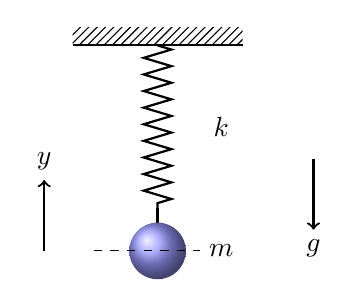
\begin{tikzpicture}[scale=0.9]
  \fill[pattern=north east lines] (-1.2,0) rectangle (1.2,0.25);
  \draw[thick] (-1.2,0) -- (1.2,0);
  \draw[thick, decorate, decoration={zigzag, segment length=6pt, amplitude=5pt}] (0,0) -- (0,-2.3);
  \draw[thick] (0,-2.3) -- (0,-2.5);
  \shade[ball color=blue!40] (0,-2.9) circle (0.4);
  \node at (0.9,-1.15) {$k$};
  \node at (0.9,-2.9) {$m$};
  \draw[->, thick] (-1.6,-2.9) -- (-1.6,-1.9) node[above] {$y$};
  \draw[->, thick] (2.2,-1.6) -- (2.2,-2.6) node[below] {$g$};
  \draw[dashed] (-0.9,-2.9) -- (0.6,-2.9);
\end{tikzpicture}
\caption{A ball of mass $m$ on a vertical spring of stiffness $k$ under gravity. $y$ is positive upward; $y = 0$ when the spring is unstretched.}
\label{fig:model}
\end{figure}

\section*{Time Integration}

Implement both methods below. In both, solve each time step with the \textbf{Newton--Raphson method} (residual $f$ and its derivative $J = \partial f / \partial y_{n+1}$), as in the codes from class, even though Eq.~\eqref{eq:eom} is linear.

\textbf{Implicit Euler.} Find $y_{n+1}$ such that
\begin{equation}
f = m \frac{y_{n+1} - y_n}{\Delta t^2} - m \frac{\dot{y}_n}{\Delta t} - F\!\left(y_{n+1}, \dot{y}_{n+1}\right) = 0, \qquad \dot{y}_{n+1} = \frac{y_{n+1} - y_n}{\Delta t}.
\end{equation}

\textbf{Newmark--Beta} (Chapter~6 of the course notes). Find $y_{n+1}$ such that
\begin{equation}
f = m \ddot{y}_{n+1} - F\!\left(y_{n+1}, \dot{y}_{n+1}\right) = 0,
\end{equation}
where $\ddot{y}_{n+1}$ and $\dot{y}_{n+1}$ follow from the Newmark relations
\begin{align}
y_{n+1} &= y_n + \Delta t\, \dot{y}_n + \Delta t^2 \left[ \left( \tfrac{1}{2} - \beta \right) \ddot{y}_n + \beta\, \ddot{y}_{n+1} \right], \\
\dot{y}_{n+1} &= \dot{y}_n + \Delta t \left[ (1 - \gamma)\, \ddot{y}_n + \gamma\, \ddot{y}_{n+1} \right].
\end{align}
The initial acceleration is $\ddot{y}_0 = F(y_0, \dot{y}_0) / m$. This assignment uses two choices of the parameters:
\begin{itemize}
    \item \textbf{Newmark (0.25, 0.5):} $\beta = 0.25$, $\gamma = 0.5$ (average acceleration). These are the default values in the code.
    \item \textbf{Newmark (0.5, 1.0):} $\beta = 0.5$, $\gamma = 1.0$ (fully implicit Newmark). Run it with \texttt{-{}-beta 0.5 -{}-gamma 1.0}.
\end{itemize}

\section*{Code Requirements}

\begin{enumerate}
    \item Submit \textbf{one} Python file, \texttt{NewmarkBetaAssignment.py}. Start from the template provided with this assignment, \texttt{NewmarkBetaAssignment\_\allowbreak template.py}. It contains two functions:
    \begin{itemize}
        \item \texttt{main()}: reads the command-line options, calls \texttt{simulate()}, prints the results, and saves a figure. \textbf{Do not change it.}
        \item \texttt{simulate(method, m, k, b, g, dt, T, beta, gamma)}: \textbf{you write this function.} It simulates the ball from $y(0) = 0$, $\dot{y}(0) = 0$ with \texttt{method} equal to \texttt{'euler'} (implicit Euler) or \texttt{'newmark'} (Newmark--Beta with \texttt{beta} and \texttt{gamma}; these two are ignored for implicit Euler), solving each time step with the Newton--Raphson method. It returns four \texttt{numpy} arrays, \texttt{t, y, v, E}, each of length $n + 1$ with $n = \mathrm{round}(T / \Delta t)$: the times $t_i = i\,\Delta t$, the position $y$, the velocity $\dot{y}$, and the total energy $E$ of Eq.~\eqref{eq:energy}.
    \end{itemize}
    You may add any other functions to the file and organize your code as you like.
    \item Use only \texttt{numpy}, \texttt{matplotlib}, and the Python standard library. The file must not import any other file. It must not open a window (do not call \texttt{plt.show()}); figures are saved to files.
    \item The program is run from a terminal as \texttt{python NewmarkBetaAssignment.py} followed by any of these options:

    \begin{center}
    \begin{tabular}{l l l}
    \toprule
    Option & Meaning & Default \\
    \midrule
    \texttt{-{}-method} & \texttt{euler} (implicit Euler) or \texttt{newmark} (Newmark--Beta) & \texttt{newmark} \\
    \texttt{-{}-m} & mass $m$ [kg] & 1 \\
    \texttt{-{}-k} & spring stiffness $k$ [N/m] & 10 \\
    \texttt{-{}-b} & drag coefficient $b$ [N$\cdot$s/m] & 0 \\
    \texttt{-{}-g} & gravity $g$ [m/s$^2$] & 9.81 \\
    \texttt{-{}-dt} & time step $\Delta t$ [s] & 0.01 \\
    \texttt{-{}-T} & total time $T$ [s] & 20 \\
    \texttt{-{}-beta}, \texttt{-{}-gamma} & Newmark parameters $\beta$, $\gamma$ & 0.25, 0.5 \\
    \bottomrule
    \end{tabular}
    \end{center}

    \item Each run prints one line with the final position, final velocity, and the initial and final energies, e.g.,
    \begin{center}
    \scriptsize\texttt{method=euler m=1 k=10 b=0 dt=0.01 T=20 y\_final=... v\_final=... E\_initial=... E\_final=...}
    \end{center}
    and saves a figure with two plots, $y$ vs.\ $t$ (with the exact solution when $b = 0$) and $E$ vs.\ $t$. \texttt{main()} already does this.
    \item The instructor will run, for example:
\begin{verbatim}
python NewmarkBetaAssignment.py --method euler --k 0
python NewmarkBetaAssignment.py --method newmark --k 0
python NewmarkBetaAssignment.py --method euler
python NewmarkBetaAssignment.py --method newmark
python NewmarkBetaAssignment.py --method newmark --b 0.5
python NewmarkBetaAssignment.py --method newmark --beta 0.5 --gamma 1.0
\end{verbatim}
    Each command should finish in a few seconds.
\end{enumerate}

\section*{Report}

Submit a report, \texttt{NewmarkBetaReport.pdf}, of \textbf{at most 5 pages}, with your name on the first page.

\textbf{Methods.} Compare three methods: \textbf{implicit Euler}, \textbf{Newmark (0.25, 0.5)} ($\beta = 0.25$, $\gamma = 0.5$), and \textbf{Newmark (0.5, 1.0)} ($\beta = 0.5$, $\gamma = 1.0$). All runs use $b = 0$.

\textbf{Figures.} Every plot must have an $x$-label and a $y$-label, with units where applicable (e.g., $t$ [s], $y$ [m], $E$ [J]), and a legend when it shows more than one curve. Number every figure, and discuss every figure in the text (e.g., ``Figure~2 shows \ldots'').

The report should have the following five sections.
\begin{enumerate}
    \item \textbf{Model and Algorithm.} Write the equation of motion and the total energy, and explain why the energy is constant when $b = 0$. Write the residual $f$ and its derivative $J = \partial f / \partial y_{n+1}$ for implicit Euler and for Newmark--Beta (with general $\beta$ and $\gamma$), and give pseudocode for one time step of each.
    \item \textbf{Verification with free fall} ($k = 0$). Plot $y$ vs.\ $t$ for the three methods together with the exact solution $y = -\frac{1}{2} g t^2$, and report $y(T)$ from each method and from the exact solution. Explain why both Newmark choices match the exact solution (up to round-off) while implicit Euler does not.
    \item \textbf{Undamped spring} ($k = 10\,\mathrm{N/m}$). Plot $y$ vs.\ $t$ (with the exact solution) and $E$ vs.\ $t$ for the three methods. Explain the differences between them.
    \item \textbf{Time step} ($k = 10\,\mathrm{N/m}$). Run the three methods with $\Delta t = 0.04$, $0.02$, and $0.01\,\mathrm{s}$, and give a table of the final energy $E(T)$ (nine values). How does the energy of each method depend on $\Delta t$?
    \item \textbf{Conclusion.} Summarize your findings. When would you use each method in a simulation of a flexible structure (e.g., the cantilever from class)?
\end{enumerate}

\section*{Generative AI}

As stated in the syllabus, you may use large language models (LLMs) and other generative AI tools to help write code. However, you are responsible for every line of code you submit and must be able to explain it when asked in person.

\textbf{Academic integrity:} this is an individual assignment. You are responsible for everything in your code and report. Including code, equations, results, or other content that you cannot explain when asked in person will be treated as a violation of academic integrity.

\end{document}
